\documentclass[12pt,a4paper]{article}

\usepackage{geometry}
\geometry{
    left=2cm, 
    right=2cm,
    top=3cm,  
    bottom=2cm
}

\usepackage[english,spanish]{babel}
\usepackage[utf8]{inputenc}
\usepackage{amsmath}

\usepackage{graphicx}
\usepackage{wrapfig}

\usepackage{csquotes}
\usepackage{hyperref}
\usepackage[style=ieee]{biblatex}
\addbibresource{referencias.bib}

\usepackage{setspace}
\setstretch{1.5}
\setlength{\parindent}{0pt}

\usepackage{enumitem}

\usepackage{xcolor}

\begin{document}
\begin{titlepage}
    \begin{minipage}[c]{0.1\textwidth}
        
\includegraphics[width=\textwidth]{Resources/logo_unam.jpg}
    \end{minipage}
    \begin{minipage}{0.8\textwidth}
        \centering
        {\Large\textbf{Universidad Nacional Autónoma de México}\\}
        {\large\textbf{Escuela Nacional de Estudios Superiores\\\underline{Unidad Morelia}}}
    \end{minipage}
    \begin{minipage}[c]{0.1\textwidth}
        
\includegraphics[width=\textwidth]{Resources/logo_enes.jpg}
    \end{minipage}
    \vspace{3cm}

    \centering
    {\large{Ante Proyecto de:\\}}
    {\Large\textbf{Análisis Estadístico de Valores Nutricionales por Tipo de Dieta}}
    \vspace{2cm}

    {{PRESENTA:\\}}
    {\large\textbf{Alexis Uriel Aguilar Uribe}}
    \vspace{1cm} 

    {{PROFESORES:\\}}
    {\large\textbf{Dra.\ María Del Río Francos}}\\
    {\large\textbf{Dr.\ César Andrés Torres Miranda}}
    \vspace{2cm}

    {{GRADO\\}}
    {\large\textbf{Licenciatura en Tecnologías para la Información en Ciencias}}
    \vspace{2cm}

    \flushleft{
    {\textbf{Asignatura:\ }Estadística Descriptiva e Inferencial}
    \vspace{2cm}}

    \flushright{
    {\textbf{A:\ }\underline{4 de Abril del 2025}}}
    \vfill
\end{titlepage}

\newpage

\tableofcontents

\newpage

\section{Presentación de los Datos}

    \subsection{Fuente de Datos}
    El conjunto de datos con el que se está trabajando para este trabajo 
    se encuentra en \cite{dataset_macronutrients}, publicado por la comunidad 
    de Kaggle. Los datos consisten de un conjunto de recetas de diferentes 
    dietas y cocinas, además incluye información de los macronutrientes que 
    aporta cada receta.\\
    \cite{dataset_macronutrients} Aunque en la descripción ni en los metadatos del conjunto de datos se 
    haga mención de las fuentes explícitas de los datos ni el objetivo de 
    esta extracción, sí cuenta con una sección de cómo usar el conjunto de 
    datos, ideas de investigación y reconocimientos.\\
    De los apartados de cómo usar el conjunto de datos e ideas de investigación, 
    se encuentra una idea, implícita, de la información que se quería estudiar. 
    La principal información de interés se vuelve que es: el crear planes 
    alimenticios saludables, ya sea usando las recetas proporcionadas o creando 
    unas nuevas basadas en una dieta y cocina, y el estudiar la relación entre 
    dieta y salud.\\
    Del apartado de reconocimientos, se concluye que las recetas fueron 
    proporcionadas por diferentes creadores de las mismas y demás contribuidores 
    al conjunto de datos. 

    \subsection{Interés del Estudio}
    Se consultó \cite{marvastipopular} en sus 
    capítulos 4 y 8, de donde se proporciona un mejor entendimiento de la 
    importancia de los macronutrientes y una descripción general de las 
    dietas en este trabajo, resultando interesante que en cada dieta se 
    consumen diferentes alimentos y productos con ciertas características 
    para ya sea respetar alguna creencia, fundamento o cuota de macronutrientes. 
    De esto último, proporciona un indicio de que existe una diferencia entre 
    las dietas a nivel de sus aportes nutricionales, por lo tanto, lo que se 
    quiere realizar es probar esta diferencia de manera significativa haciendo 
    uso de la estadística.

    \subsection{Variables del Conjunto de Datos}
    El conjunto de datos consta de las siguientes variables. Se menciona su 
    nombre, el tipo de variable y sus valores (en total y únicos):
    \begin{center}
        \begin{tabular}{|c|c|c|c|c|}
            \hline
            Variable & Nombre & Tipo & Cantidad de Datos & Valores Únicos\\
            \hline
            1 & Diet\_type & Cualitativa Nominal & 7806 & 5 \\
            2 & Recipe\_name & Cualitativa Nominal & 7806 & 7062\\
            3 & Cuisine\_type & Cualitativa Nominal & 7806 & 19\\
            4 & Protein(g) & Cuantitativa Continua & 7806 & 6060\\
            5 & Carbs(g) & Cuantitativa Continua & 7806 & 6618\\
            6 & Fat(g) & Cuantitativa Continua & 7806 & 6322\\
            \hline
        \end{tabular}
    \end{center}
    La variable \emph{Recipe\_Name} no es relevante para este trabajo pero figura 
    dentro del dataset. Se hace mención que el conjunto de datos no presenta 
    valores faltantes.

\newpage

\section{Estadística Descriptiva}
    Debido a que cada receta puede aportar una amplia variedad de valores 
    en sus macronutrientes, esto podría dificultar la comparación entre 
    los aportes nutricionales de las dietas. Por ello, para reducir este 
    sesgo, se aplico una normalización a los valores, es decir, 
    los macronutrientes de cada receta se dividió por el total de macronutrientes 
    que aportaba la receta, para así manejar los aportes proporcionales de 
    cada macronutriente en cada una de las recetas. De aquí en adelante, cuando 
    se mencionan los aportes nutricionales o por macronutriente de una receta, 
    siempre se hace referencia a estos aportes proporcionales respecto al total de 
    macronutrientes en una receta. 

    \subsection{Descripción de los Valores de las Variables}
    Para el presente trabajo se harán uso de las siguientes variables, se 
    acompañan con una descripción de su significado:
    \begin{itemize}[label=\textbullet]
        \item \textbf{Diet\_type}: Variable que representa el tipo de 
        dieta (DASH, keto, mediterránea, paleo, vegana) a la que 
        pertenece una receta. Con esta variable se va permitir estratificar 
        las recetas y estudiarlas de una manera más granular, es decir, 
        por tipo de dieta para llegar a conformar hipótesis sobre lo qué 
        está pasando en una dieta o entre las diferentes dietas.
        \item \textbf{Cuisine\_type}: Variable que representa a qué (estilo 
        de) cocina o región (mexicana, americana, italiana, entre otras) pertenece una 
        receta. Al usarla va a permitir el comparar cómo son las recetas 
        de una dieta en diferentes regiones, en específico el 
        como se compara la dieta mediterránea en el mediterráneo  
        contra otras regiones geográficas.
        \item \textbf{Protein(g)}: Después de la transformación, representa el 
        porcentaje, respecto al total de macronutrientes, de proteínas que son 
        aportados por una receta. El usar las proteínas va a permitir la 
        comparación entre diferentes dietas, siendo esto el eje central del trabajo
        \item \textbf{Carbs(g)}: Después de la transformación, representa el 
        porcentaje, respecto al total de macronutrientes, de carbohidratos que 
        son aportados por una receta. Siendo otro de los macronutrientes de una 
        comida, se vuelve relevante para la comparación entre recetas y dietas.
        \item \textbf{Fat(g)}: Después de la transformación, representa el 
        porcentaje, respecto al total de macronutrientes, de grasas que son 
        aportados por una receta. Y el último macronutriente, como en los 
        anteriores, se vuelve una variable relevante para la comparación entre dietas.
    \end{itemize}

    \subsection{Medidas de Tendencia Central y Dispersión}
    Realizando el resumen de las medidas, se tiene:
    \begin{center}
        \begin{tabular}{|c|ccc|}
            \hline
            Medida & Carbs(g) & Protein(g) & Fat(g) \\
            \hline
            Media               & 0.433471 & 0.234762 & 0.331767 \\
            $Q_1$               & 0.205251 & 0.110188 & 0.184583 \\
            $Q_2$               & 0.432028 & 0.190931 & 0.314359 \\
            $Q_3$               & 0.635058 & 0.338059 & 0.464532 \\
            Desviación Estándar & 0.256032 & 0.163886 & 0.194920 \\
            Mínimo              & 0.000330 & 0.000000 & 0.000000 \\
            Máximo              & 1.000000 & 0.887557 & 0.997940 \\
            Asimetría de Fisher & 0.189556 & 0.922401 & 0.461455 \\
            \hline
        \end{tabular}
    \end{center}
    Debido a que son medidas sobre todos los datos, sin estratificar, 
    se tiene que no hay una referencia de lo que se espera obtener y 
    parte de la información que contienen queda diluida o desvanecida. 
    Esto debido a que las dietas como la vegana es baja en proteínas y 
    la keto en carbohidratos \cite{marvastipopular}, por lo que cualquier 
    suposición no se podría sostener sobre todos las dietas.\\

    Aún así, se reportan bajos valores en proteínas en comparación 
    con los carbohidratos y grasas si se hace uso de la mediana ($Q_2$), 
    dicho así: el cincuenta por ciento de las recetas tienen a lo mucho  
    $19.09\%$ de proteínas, en comparación con el $43.20\%$ de carbohidratos 
    y el $31.43\%$ de grasas. Esto es un indicio de que las recetas, en general, 
    tienden a ser altas en carbohidratos y grasas entre las diferentes dietas y 
    cocinas; mientras que son bajas en proteínas.\\
    Este último punto puede ser apoyado si se considera la media de los 
    macronutrientes, que siguen esta tendencia de aportes.\\

    Si se gráfica la distribución de los macronutrientes se tiene que, debido 
    a la asimetría y a la desviación estándar, contienen datos atípicos en proteínas y grasas en una región 
    positiva respecto a la mediana, y esto se relaciona con lo mencionado de que 
    una receta no tiende a un aporte alto de proteínas. Y si se consider el rango 
    intercuartil, se observa que en estos macronutrientes es menor, en comparación, 
    que con el de los carbohidratos, esto muestra como los valores de proteínas y 
    grasas se encuentran concentradas en ciertas regiones en contraste con los posibles 
    valores de los carbohidratos que son más diversos.
    \begin{center}
        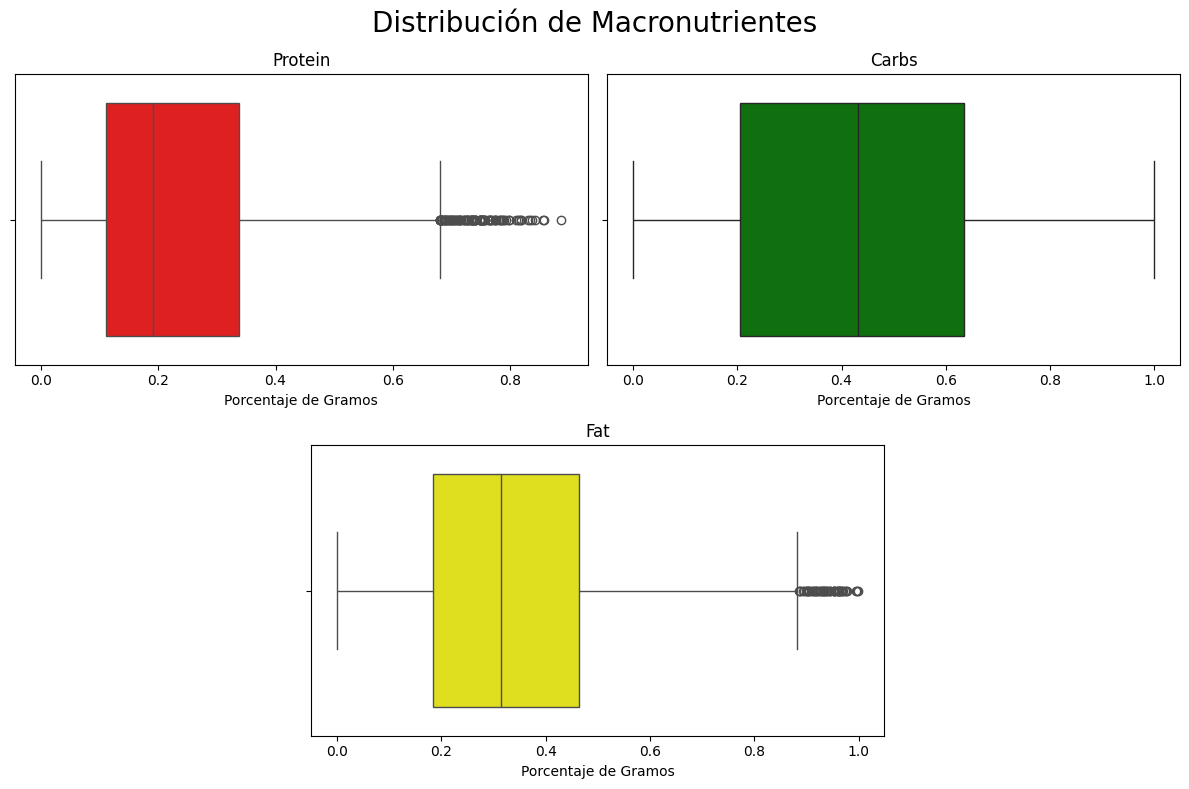
\includegraphics[width=0.75\textwidth]{Resources/2_02_plot_01.png}
    \end{center}

    Debido a que existe la presencia de datos atípicos, lo más adecuado es tratarlos 
    de manera estratificada, por tipo de dieta. Esto debido a que tratarlos de manera 
    general podría evocar que ciertas dietas queden menos representadas en comparación 
    con otras o que incluso se pierda información para consecuentes procesos. Y al 
    tratar los valores atípicos dentro de cada dieta permite reducir el impacto de 
    perder información valiosa y se siga conservando las recetas relevantes para una dieta.

    \subsection{Estratificación de Valores Cuantitativos}
    La variable \emph{Diet\_type} es la principal que se emplea para la 
    estratificación de las recetas, debido a que permite seprarlas 
    según una criterio bien definida, a qué dieta pertenecen. Para cada 
    una de las cinco dietas se presentan los datos tabulados de sus 
    medidas de tendencia central y dispersión junto con su histograma 
    de los valores en sus macronutrientes.\\

    \subsubsection{Dieta DASH}
        Una receta de esta dieta tendrá que, en promedio, el $55\%$ de sus 
        macronutrientes son carbohidratos (provenientes de frutas, vegetales 
        y granos enteros); el $25\%$ son grasas que, por su naturaleza, son 
        saludables; y el $20\%$ son proteínas, las cuáles provienen de carnes margas.\\
        Aunque esta dieta se menciona ser saludable para la salud cardiovascular, 
        no implica que exista un balance o equilibrio en los macronutrientes 
        consumidos por receta.\\

        El cincuenta por ciento de las recetas tienen entre $33\%$ y $76\%$ 
        de carbohidratos en su composición, este fenómeno se puede observar 
        también	en su desviación estándar. Esto implica que los carbohidratos 
        pueden estar en cualquier proporción pero con una tendencia a tener 
        una alta presencia.\\

        Debido a la desviación estándar y rango intercuartil de las proporciones 
        de proteínas y grasas, se tiene que estos macronutrientes se encuentran 
        concentrados en un rango más pequeño de valores en comparación con el 
        fenómeno anterior de la composición de carbohidratos. En específico, el 
        cincuenta por ciento de las recetas tienen entre el $7\%$ y $28\%$ de 
        proteínas y entre $10\%$ y $37\%$ de grasas.
        \begin{center}
            \begin{tabular}{|c|ccc|}
                \hline
                Medida & Carbs(g) & Protein(g) & Fat(g) \\
                \hline
                Media               & 0.549425 & 0.196241 & 0.254334  \\
                $Q_1$               & 0.331143 & 0.068931 & 0.103381  \\
                $Q_2$               & 0.555219 & 0.156626 & 0.234742  \\
                $Q_3$               & 0.757917 & 0.282629 &	0.371292  \\
                Desviación Estándar & 0.278850 & 0.162871 & 0.194078  \\
                Mínimo              & 0.001526 & 0.000000 & 0.000000  \\
                Máximo              & 1.000000 & 0.833467 & 0.973404  \\
                Asimetría de Fisher & -0.057984 & 1.101171 & 0.732534  \\
                \hline
            \end{tabular}
        \end{center}
        De lo mencionado, podría significar que la contribución de los macronutrientes 
        no son tan variadas como lo que se esperaría contradiciendo que sea una 
        dieta saludable, notando que es una dieta rica en carbohidratos. Esto no 
        excluye que el consumir varias recetas (comidas) se logré un balance.\\

        Debido a que existe un sesgo positivo notable en las contribuciones de 
        proteínas y grasas, se tiene que las recetas van a tender a tener bajos 
        aportes de estos macronutrientes y que si tienen un alto aporte se 
        consideraría una receta atípica dentro de la dieta, de manera estadística. 
        Lo primero refleja un posible imbalance en el consumo de macronutrientes, 
        contradiciendo que sea una dieta saludable para la salud cardiovascular.
        \begin{center}
            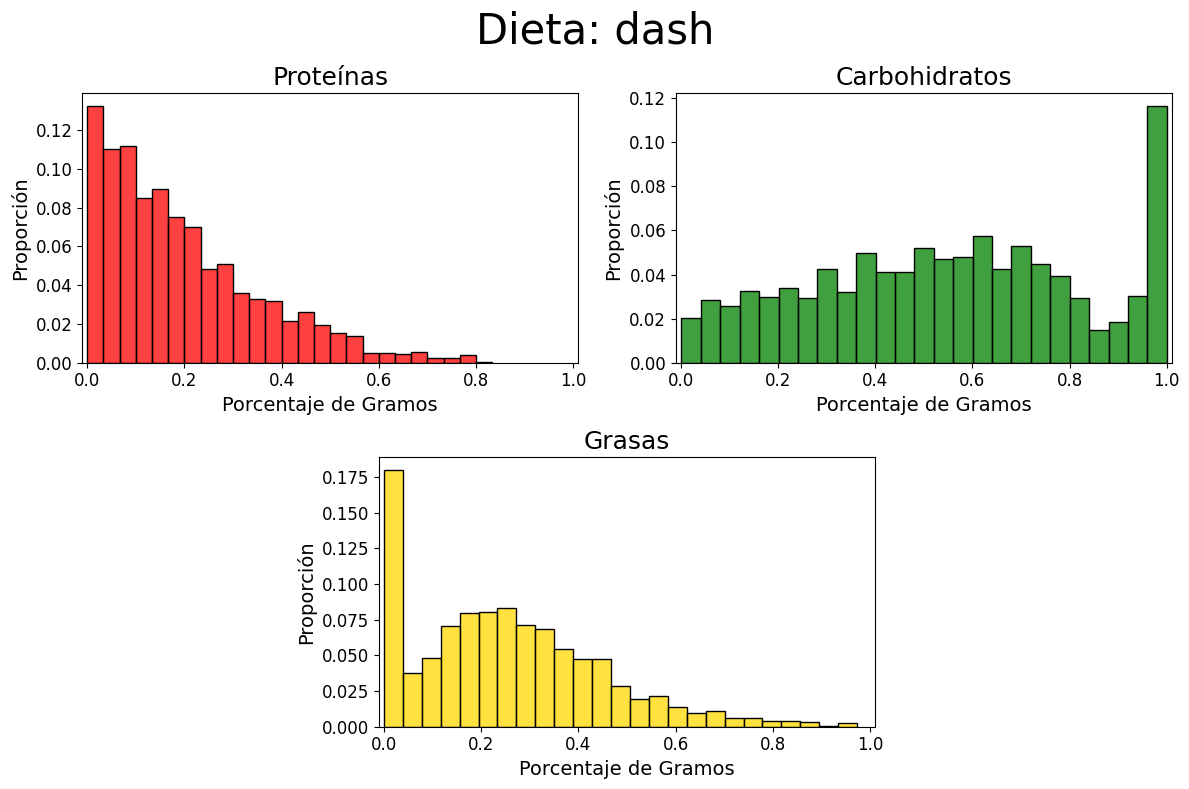
\includegraphics[width=0.75\textwidth]{Resources/2_03_plot_01.png}
        \end{center}

    \subsubsection{Dieta Keto}
        Una receta de esta dieta tendrá que, en promedio, el $50\%$ de 
        sus macronutrientes son grasas, esto se relaciona con el hecho de 
        que se intenta inducir la ketosis (principio en que se basa esta         
        dieta); el $30\%$ son proteínas, notando que se intenta reducir 
        el consumo de carbohidratos; y el $20\%$ son carbohidratos, 
        resaltando ser una dieta baja en carbohidratos.\\

        El cincuenta por ciento de las recetas tienen entre el $40\%$ y 
        $60\%$ de grasas en su composición, denotando que existe una alta 
        concentración de recetas con una alta composición en grasas. Y, de 
        igual manera, el cincuenta por ciento de las recetas tienen entre 
        el $8\%$ y $26\%$ de carbohidratos, verificándose el hecho de que 
        se quiere minimizar el consumo de carbohidratos.\\

        En las proteínas, se puede observar que es como un caso intermedio, 
        debido a que, usando su rango intercuartil, la distribución de valores 
        que toma es amplia pero sigue siendo valores menores a los que se puede 
        encontrar en grasas. Esto es consecuencia de que se quiere intentar 
        eliminar el consumo de carbohidratos mientras se incrementa el consumo 
        de grasas.
        \begin{center}
            \begin{tabular}{|c|ccc|}
                \hline
                Medida & Carbs(g) & Protein(g) & Fat(g) \\
                \hline
                Media               & 0.200879 & 0.301777 & 0.497344  \\
                $Q_1$               & 0.085517 & 0.158284 & 0.405354  \\
                $Q_2$               & 0.157348 & 0.302900 & 0.505751  \\
                $Q_3$               & 0.267535 & 0.409453 & 0.591887  \\
                Desviación Estándar & 0.160609 & 0.167027 & 0.166572  \\
                Mínimo              & 0.002060 & 0.000000 & 0.000000  \\
                Máximo              & 1.000000 & 0.856868 & 0.997940  \\
                Asimetría de Fisher & 1.634945 & 0.314795 & -0.147406 \\
                \hline
            \end{tabular}
        \end{center}
        Como los tres macronutrientes reportan una desviación estándar similar, 
        se tiene que es indicio de que las recetas son similares en su composición 
        de macronutrientes, es decir, diferentes recetas reportan composiciones 
        semejantes pero que se conforman de distintos alimentos o productos.\\

        Como la proporciones de carbohidratos cuenta con un sesgo positivo, se 
        tiene que refuerza el hecho de ser una dieta baja en carbohidratos. 
        De los aportes de grasas, se observa que su sesgo es despreciable implicando 
        que existen recetas tanto con aportes altos de este macronutriente (lo que se 
        busca) mientras que hay recetas con una contribución baja o nula del mismo.
        \begin{center}
            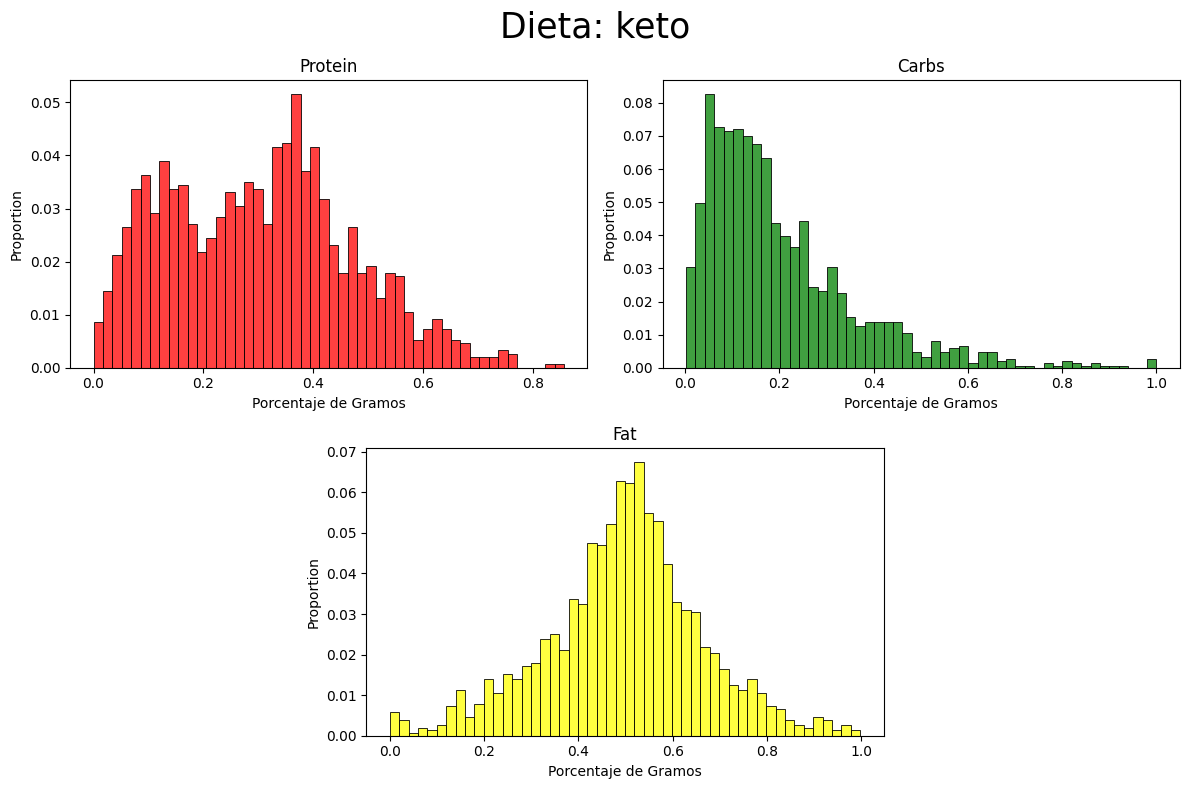
\includegraphics[width=0.75\textwidth]{Resources/2_03_plot_02.png}
        \end{center}

    \subsubsection{Dieta Mediterránea}
        Una receta de esta dieta tendrá que, en promedio, el $42\%$ de sus 
        macronutrientes son carbohidratos, esto debido a un alto consumo de 
        productos como, frutas, vegetales y granos enteros; el $30\%$ son 
        grasas, resaltando un alto consumo de nueces y aceite de oliva, como 
        también un consumo moderado de pescado; y el $28\%$ son proteínas, 
        vinculado con un consumo moderado de pescado y aves de corral, y un 
        bajo consumo de carnes rojas.\\

        El cincuenta por ciento de las recetas tienen entre el $25\%$ y $60\%$ 
        de carbohidratos en sus aportes, reflejando una alta variedad de composiciones 
        sobre este macronutriente. Esto debido a los alimentos base de esta dieta y 
        al valor reportada para su desviación estándar,haciendo posible esta 
        diversidad de valores.\\

        En el caso de las proteínas y grasas, muestras distribuciones que siguen 
        patrones similares en el sentido de que sus desviaciones estándar y rangos 
        intercuartiles son similares. Por lo que las recetas, por al menos en estos 
        macronutrientes, tienen composiciones similares. Específicamente, el cincuenta 
        por ciento de ellas tiene entre el $16\%$ y $38\%$ de proteínas	y el $18\%$ y 
        $39\%$ de grasas en la composiciones de estos macronutrientes.
        \begin{center}
            \begin{tabular}{|c|ccc|}
                \hline
                Medida & Carbs(g) & Protein(g) & Fat(g) \\
                \hline
                Media               & 0.424493 & 0.279357 & 0.296150  \\
                $Q_1$               & 0.249955 & 0.159633 & 0.180357  \\
                $Q_2$               & 0.439382 & 0.227883 & 0.268336  \\
                $Q_3$               & 0.607531 & 0.377820 & 0.390404  \\
                Desviación Estándar & 0.214325 & 0.162853 & 0.160783  \\
                Mínimo              & 0.006733 & 0.005036 & 0.001731  \\
                Máximo              & 0.992746 & 0.887557 & 0.968722  \\
                Asimetría de Fisher & -0.096055 & 0.955922 & 0.869493 \\
                \hline
            \end{tabular}
        \end{center}
        La amplia variedad en la composición de macronutrientes en las recetas podría 
        estar relacionada con la internacionalización de esta dieta, en específico, de 
        tomar inspiración de recetas y adaptarlas a los productos disponibles en 
        ciertas regiones geográficas.\\

        La proporción de proteínas está segada positivamente y junto con una 
        alta acumulación de recetas con bajo porcentaje de proteínas, se tiene que 
        esta dieta figura como una con bajo consumo de alimentos ricos en proteínas. 
        \begin{center}
            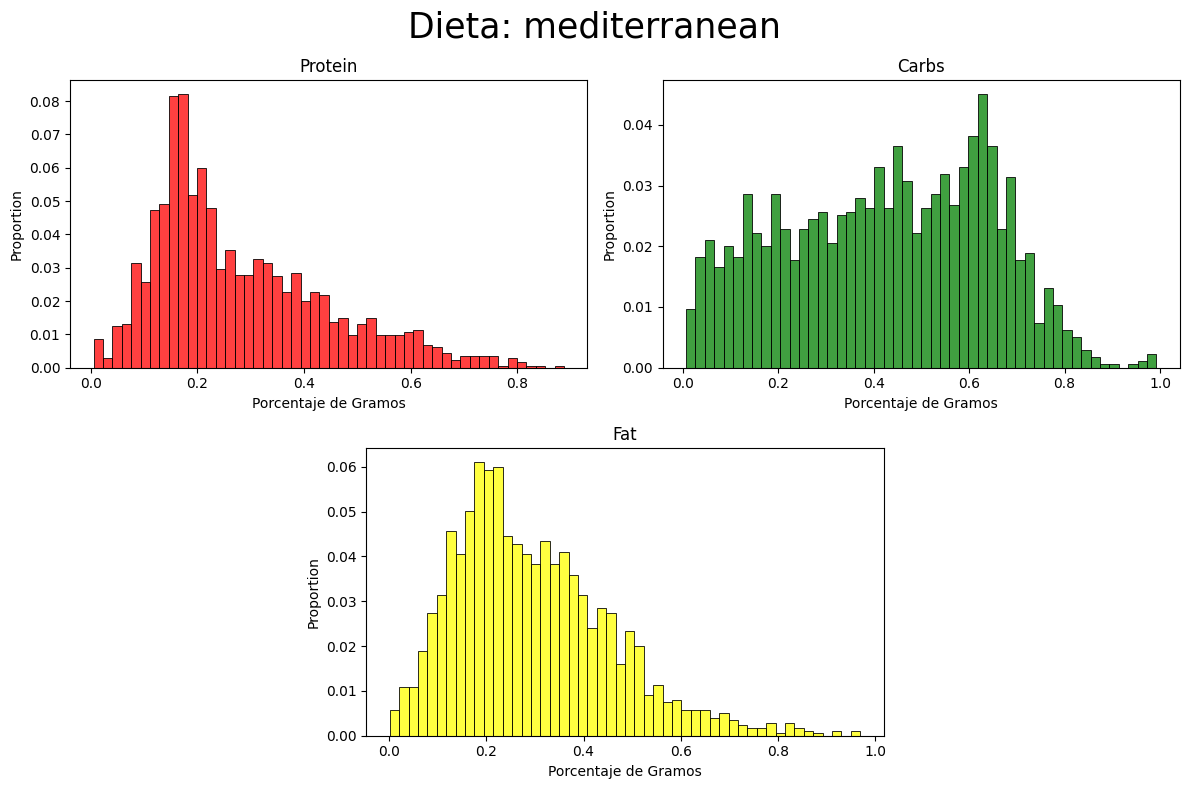
\includegraphics[width=0.75\textwidth]{Resources/2_03_plot_03.png}
        \end{center}

    \subsubsection{Dieta Paleo}
        Una receta de esta dieta tendrá que, en promedio, el $38\%$ de sus 
        macronutrientes son grasas y el $37\%$ son carbohidratos, esto se 
        relaciona con el consumo de productos como frutas, vegetales, nueces 
        y semillas; y el $25\%$ son proteínas cuyas principales fuentes son 
        carnes margas y pescado.\\

        El cincuenta por ciento de las recetas tienen entre el $19\%$ y $51\%$ 
        de carbohidratos en sus aportes, indicando una alta variedad de recetas 
        respecto a este macronutriente, esto se debe al consumo de alimentos que 
        se encuentran en la naturaleza o en estado salvaje (excluyendo algunos 
        de ellos).\\

        Como las proteínas y grasas tienen desviaciones estándar similares, refleja 
        que los alimentos y productos asociados a estos macronutrientes no tengan 
        una alta diversidad. Es decir, las recetas tienen muchos productos y alimentos 
        en común. En cambio, sus rangos intercuartiles difieren, mostrando como 
        las proteínas, sus valores, están más concentradas en un rango menor en 
        comparación con el de las grasas.
        \begin{center}
            \begin{tabular}{|c|ccc|}
                \hline
                Medida & Carbs(g) & Protein(g) & Fat(g) \\
                \hline
                Media               & 0.371307 & 0.249693 & 0.379000  \\
                $Q_1$               & 0.192399 & 0.102963 & 0.256579  \\
                $Q_2$               & 0.351300 & 0.205532 & 0.382447  \\
                $Q_3$               & 0.515054 & 0.375392 & 0.488116  \\
                Desviación Estándar & 0.221506 & 0.175031 & 0.175471  \\
                Mínimo              & 0.003612 & 0.000000 & 0.001404  \\
                Máximo              & 0.987368 & 0.858503 & 0.968835  \\
                Asimetría de Fisher & 0.488656 & 0.711408 & 0.312673  \\
                \hline
            \end{tabular}
        \end{center}
        La posible limitante de alimentos asociados a proteínas	y grasas 
        podría impactar en que las recetas estén hechas con los mismos productos 
        dentro de la misma región geográfica. Estos se relacionaría con una 
        baja variedad en la presencia de estos macronutrientes.\\

        Se observa como las recetas tienden a tener una contribución moderada de 
        carbohidratos y grasas, esto se relaciona con los principales alimentos 
        que son consumidos en esta dieta. Mientras que sus aportes de proteínas 
        son bajas en comparación con los otros dos macronutrientes.
        \begin{center}
            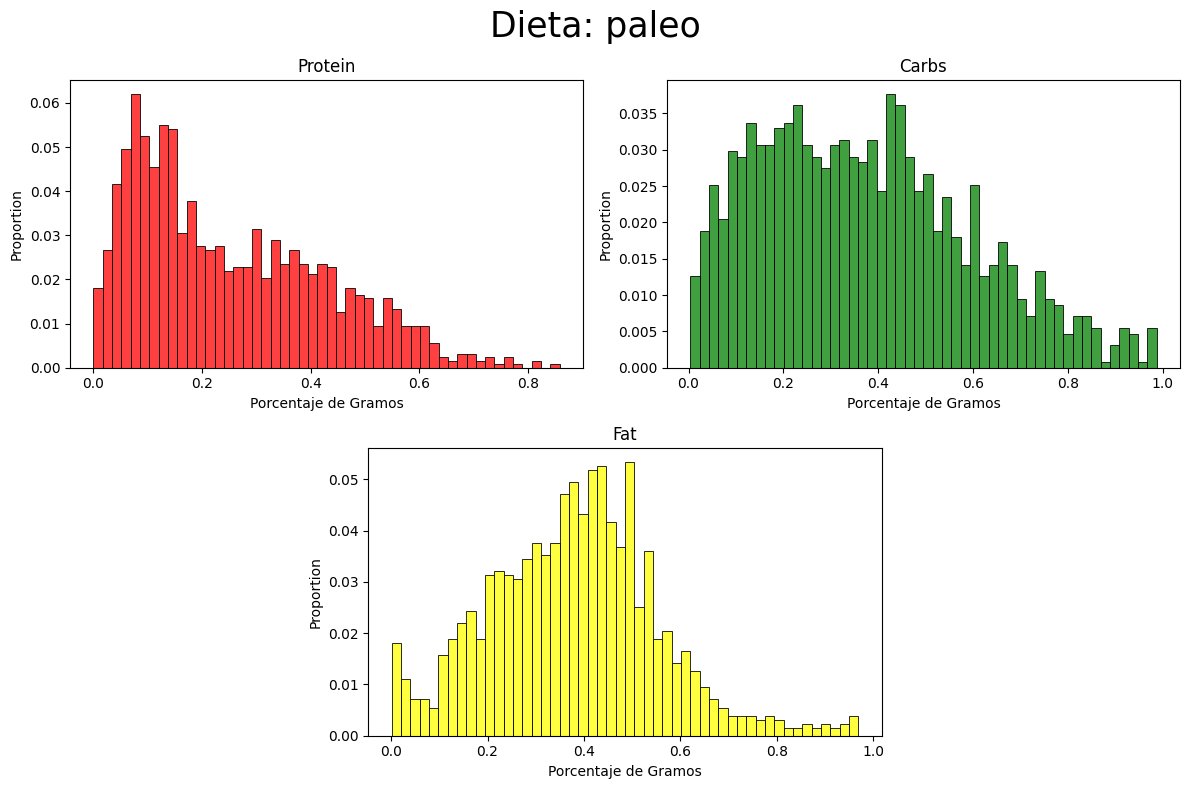
\includegraphics[width=0.75\textwidth]{Resources/2_03_plot_04.png}
        \end{center}

    \subsubsection{Dieta Vegana}
        Una receta de esta dieta tendrá que, en promedio, el $60\%$ de 
        sus macronutrientes son carbohidratos, que provienen de fuentes 
        como vegetales, frutas, cereales y legumbres; el $25\%$ son grasas, 
        relacionadas con el consumo de nueces y semillas; y el $15\%$ son 
        proteínas, esto debido a un nulo consumo de alimentos de origen 
        animal y que estas fuentes son reemplazadas por fuentes vegetales.
        \begin{center}
            \begin{tabular}{|c|ccc|}
                \hline
                Medida & Carbs(g) & Protein(g) & Fat(g) \\
                \hline
                Media               & 0.593968 & 0.148489 & 0.257543  \\
                $Q_1$               & 0.504070 & 0.085339 & 0.142575  \\
                $Q_2$               & 0.626246 & 0.139688 & 0.231518  \\
                $Q_3$               & 0.714679 & 0.190381 & 0.344529  \\
                Desviación Estándar & 0.171203 & 0.086088 & 0.160277  \\
                Mínimo              & 0.000330 & 0.001921 & 0.000112  \\
                Máximo              & 0.986872 & 0.647416 & 0.994887  \\
                Asimetría de Fisher & 0.189556 & 0.922401 & 0.461455  \\
                \hline
            \end{tabular}
        \end{center}
        De las proporciones de proteínas, se resalta una alta acumulación de 
        recetas con bajos aportes de proteínas, esto hace de esta dieta una 
        con bajo consumo de proteínas. Lo último debido a que las principales 
        fuentes proteínas son animales y haciendo que los aportes de carbohidratos 
        sean altos en comparación con los otros dos macronutrientes.
        \begin{center}
            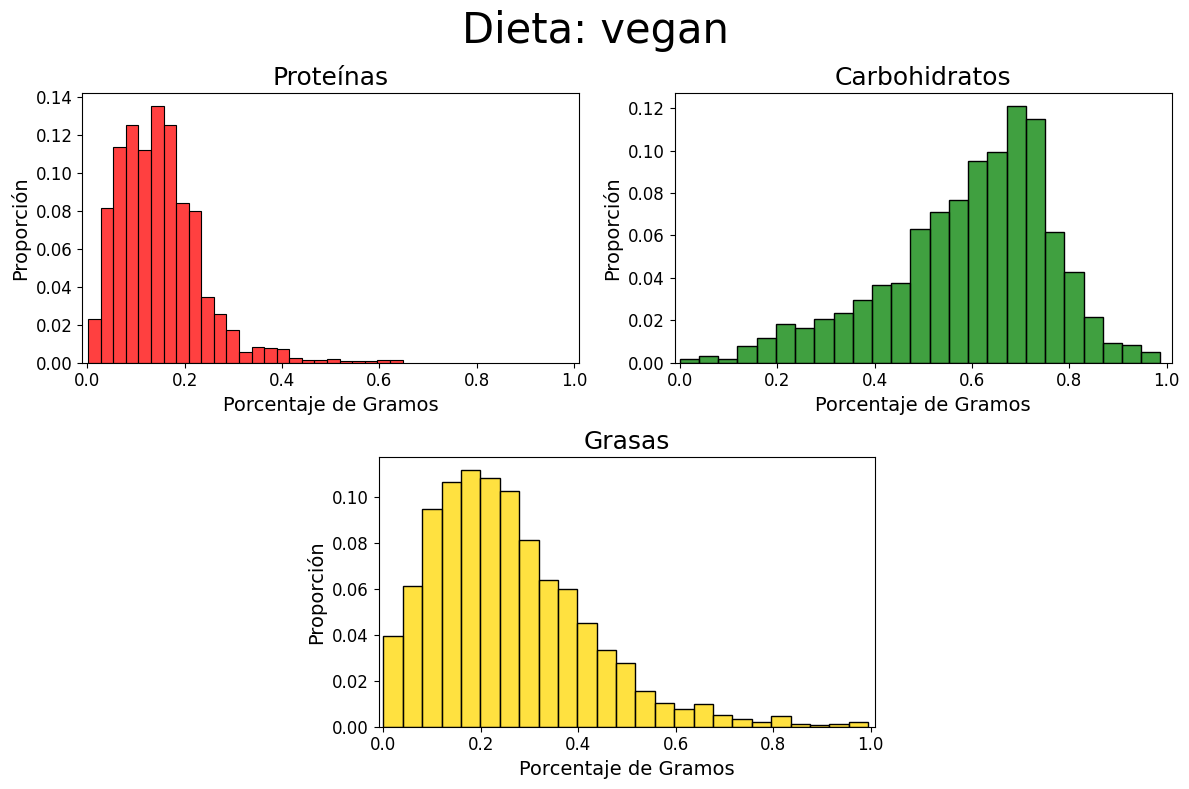
\includegraphics[width=0.75\textwidth]{Resources/2_03_plot_05.png}
        \end{center}

    \subsubsection{Gráfico de Cajas y Bigotes de la distribución de Macronutrientes por Dieta}
        Se anexan las gráficas de cajas y bigotes de las distribuciones de los 
        macronutrientes por dieta para apoyar las observaciones realizadas anteriormente.
        \begin{center}
            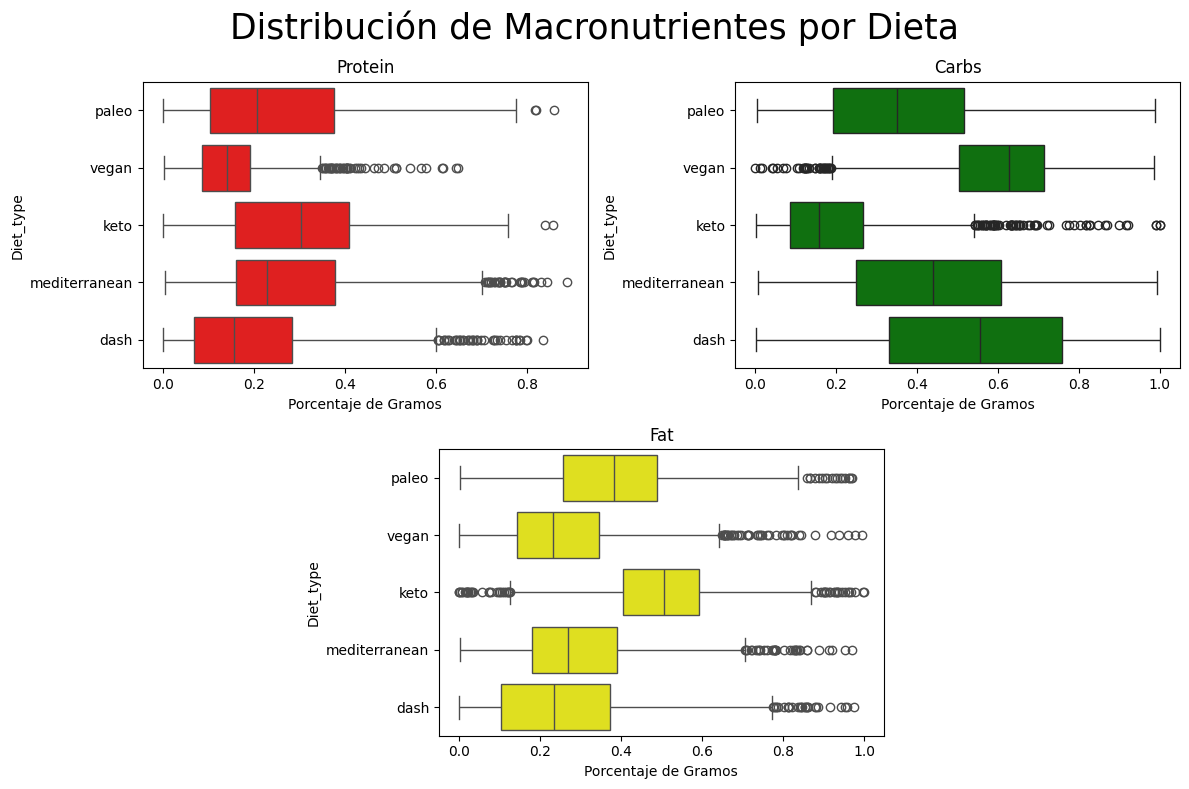
\includegraphics[width=0.75\textwidth]{Resources/2_03_plot_06.png}
        \end{center}

\newpage

\section{Muestreo e Intervalos de Confianza}
    Como las tres variables cuantitativas tienen el mismo nivel 
    de relevancia, se opta por usar los Carbs(g) como atributo 
    para el Muestreo. Y para ambos muestreos se realizan de 
    tamaño $50$ y, usando la Regla de Sturges, se emplean 7 clases 
    o bins para la tabla de frecuencias.
    
    \subsection{Muestreo Aleatorio Simple}
        
    \subsubsection{Resultados del Muestreo}
        \begin{center}
            \begin{tabular}{ccccc}
                0.17269271 & 0.46650541 & 0.75534765 & 0.47087379 & 0.63277125 \\
                0.07006336 & 0.05484247 & 0.65481006 & 0.16118891 & 0.2385986  \\
                0.4684997  & 0.24332505 & 0.62191414 & 0.34102783 & 0.62236612 \\
                0.39206706 & 0.08786462 & 0.37490208 & 0.03025985 & 0.46368715 \\
                0.50368913 & 0.25911022 & 0.64134393 & 0.62119952 & 0.67296013 \\
                0.69099174 & 0.5093633  & 0.3897762  & 0.50870391 & 0.62610896 \\
                0.16637611 & 0.00205997 & 0.83795162 & 0.70500232 & 0.39452352 \\
                0.96228571 & 0.3650539  & 0.73331589 & 0.2995115  & 0.17188455 \\
                0.7579386  & 0.35745213 & 0.5351373  & 0.68094919 & 0.19350238 \\
                0.32026529 & 0.62170193 & 0.13598024 & 0.96879183 & 0.30912958 \\
            \end{tabular}
        \end{center}

    \subsubsection{Z-Scores del Muestreo}
        Se tiene que la media muestral $\overline{x}$ es $0.445313$ y la 
        desviación estándar muestral $s$ es $0.246293$.
        \begin{center}
            \begin{tabular}{ccccc}
                -1.10689678 &  0.08604412 &  1.25880389 &  0.10378063 &  0.76111813 \\
                -1.52359336 & -1.58539332 &  0.85060029 & -1.15360459 & -0.83930511 \\
                 0.09414135 & -0.82011471 &  0.717036   & -0.42342106 &  0.71887111 \\
                -0.21619111 & -1.45131653 & -0.28588451 & -1.68520391 &  0.07460139 \\
                 0.23701778 & -0.75602365 &  0.79592498 &  0.71413449 &  0.92429335 \\
                 0.99750546 &  0.26005608 & -0.22549249 &  0.25737883 &  0.73406782 \\
                -1.13254349 & -1.79970131 &  1.59419324 &  1.05439133 & -0.20621739 \\
                 2.09901562 & -0.32587018 &  1.16935033 & -0.59198603 & -1.11017805 \\
                 1.2693237  & -0.35673498 &  0.36470391 &  0.95673061 & -1.02240518 \\
                -0.50772129 &  0.71617437 & -1.25595705 &  2.12543183 & -0.55293458 \\
            \end{tabular}
        \end{center}

    \subsubsection{Tabla de Frecuencias}
        \begin{center}
            \begin{tabular}{|c|c|c|c|c|}
                \hline
                Marca de Clase & Puntaje Z & Frecuencia Absoluta & Frecuencia Relativa & Frecuencia Acumulada \\
                \hline
                0.071112 & -1.519335 & 6  & 0.120000 & 0.120000 \\
                0.209217 & -0.958601 & 8  & 0.160000 & 0.280000 \\
                0.347321 & -0.397868 & 10 & 0.200000 & 0.480000 \\
                0.485426 &  0.162865 & 8  & 0.160000 & 0.640000 \\
                0.623530 &  0.723599 & 11 & 0.220000 & 0.860000 \\
                0.761635 &  1.284332 & 4  & 0.080000 & 0.940000 \\
                0.899740 &  1.845065 & 3  & 0.060000 & 1.000000 \\
                \hline
            \end{tabular}
        \end{center} 

    \subsubsection{Medidas de Tendencia Central y Dispersión Muestrales}
        \begin{center}
            \begin{tabular}{|c|c|}
                \hline
                Medida muestral & Carbs(g) \\
                \hline
                Media & 0.445313 \\
                $Q_1$ & 0.247271 \\
                $Q_2$ & 0.465096 \\
                $Q_3$ & 0.631106 \\
                Desviación Estándar & 0.246293 \\
                Mínimo & 0.002060 \\
                Máximo & 0.968792 \\
                Asimetría de Fisher & 0.077583 \\
                \hline
                \end{tabular}
        \end{center}
    
    \subsubsection{Comparativa con las Medidas Poblacionales}
        En algunas métricas como lo son la media, el primer y segundo cuartil, 
        la desviación estándar, el máximo y la asimetría muestrales 
        difieren de sus respectivos valores poblacionales. De los valores, era 
        esperado que todos difieran aunque fuera un poco, salvo la media; para 
        probar esto último sería necesario de aplicar una prueba de hipótesis.\\
        Si se compara con la distribución poblacional, se tiene que la 
        distribución se conserva hasta cierto punto.
        \begin{center}
            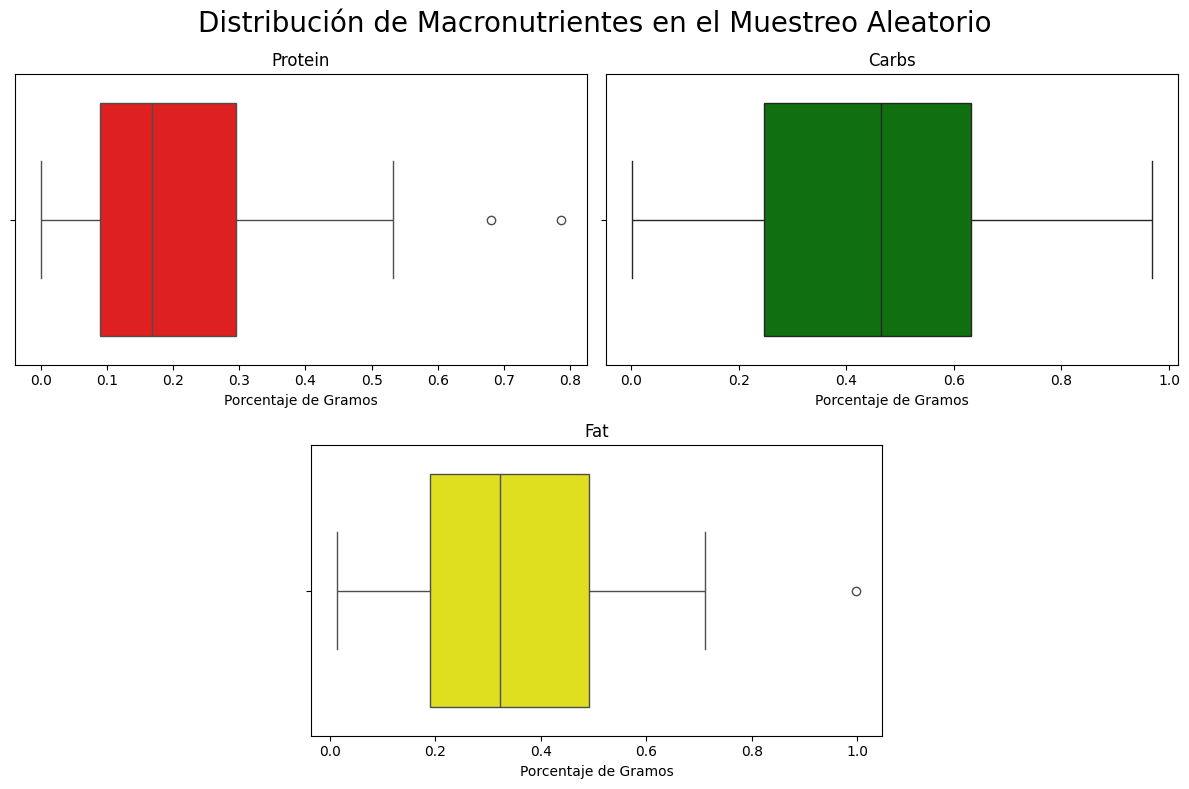
\includegraphics[width=0.75\textwidth]{Resources/3_01_plot_01.png}
        \end{center}
    
    \subsection{Muestreo Aleatorio Estratificado}

    \subsubsection{Resultados del Muestreo}
        \begin{center}
            \begin{tabular}{ccccc}
                \textcolor{magenta}{0.44793647} & \textcolor{magenta}{0.18250769} & \textcolor{magenta}{0.63935358} & \textcolor{magenta}{0.21435184} & \textcolor{magenta}{0.91825902} \\
                \textcolor{magenta}{0.70068017} & \textcolor{magenta}{0.55288489} & \textcolor{magenta}{0.49903342} & \textcolor{magenta}{0.74194743} & \textcolor{magenta}{0.39776892} \\
                \textcolor{magenta}{0.68474824} & \textcolor{orange}{0.21756679} & \textcolor{orange}{0.64524101} & \textcolor{orange}{0.11898573} & \textcolor{orange}{0.11534155} \\
                \textcolor{orange}{0.51769646} & \textcolor{orange}{0.84650821} & \textcolor{orange}{0.08359541} & \textcolor{orange}{0.24333481} & \textcolor{orange}{0.42687973} \\
                \textcolor{orange}{0.04969789} & \textcolor{cyan}{0.6525685}  & \textcolor{cyan}{0.09963134} & \textcolor{cyan}{0.13678711} & \textcolor{cyan}{0.01271082} \\
                \textcolor{cyan}{0.60119711} & \textcolor{cyan}{0.53384367} & \textcolor{cyan}{0.71907757} & \textcolor{cyan}{0.58809768} & \textcolor{cyan}{0.37297297} \\
                \textcolor{cyan}{0.61700427} & \textcolor{cyan}{0.75929204} & \textcolor{purple}{0.34345027} & \textcolor{purple}{0.15223487} & \textcolor{purple}{0.57504277} \\
                \textcolor{purple}{0.69714352} & \textcolor{purple}{0.32857582} & \textcolor{purple}{0.39527363} & \textcolor{purple}{0.19990062} & \textcolor{purple}{0.30321616} \\
                \textcolor{teal}{0.3849578}  & \textcolor{teal}{0.65746746} & \textcolor{teal}{0.69443097} & \textcolor{teal}{0.65933286} & \textcolor{teal}{0.42047204} \\
                \textcolor{teal}{0.37633321} & \textcolor{teal}{0.7136477}  & \textcolor{teal}{0.53091451} & \textcolor{teal}{0.63226859} & \textcolor{teal}{0.50493571} 
            \end{tabular}
        \end{center}
        Leyenda de colores: \textcolor{magenta}{DASH}, \textcolor{orange}{Keto}, \textcolor{cyan}{Mediterránea}, 
        \textcolor{purple}{Paleo} y \textcolor{teal}{Vegana}.

    \subsubsection{Z-Scores del Muestreo}
        Se tiene que la media muestral $\overline{x}$ es $0.458142$ y la 
        desviación estándar muestral $s$ es $0.233125$.
        \begin{center}
            \begin{tabular}{ccccc}
                \textcolor{magenta}{-0.04377718} & \textcolor{magenta}{-1.18234679} & \textcolor{magenta}{ 0.77731576} & \textcolor{magenta}{-1.04574978} & \textcolor{magenta}{ 1.97369417} \\
                \textcolor{magenta}{ 1.04037915} & \textcolor{magenta}{ 0.40640414} & \textcolor{magenta}{ 0.17540563} & \textcolor{magenta}{ 1.21739704} & \textcolor{magenta}{-0.2589733}  \\
                \textcolor{magenta}{ 0.97203835} & \textcolor{orange}{-1.03195909} & \textcolor{orange}{ 0.80257021} & \textcolor{orange}{-1.45482732} & \textcolor{orange}{-1.47045922} \\
                \textcolor{orange}{ 0.25546167} & \textcolor{orange}{ 1.66591559} & \textcolor{orange}{-1.60663578} & \textcolor{orange}{-0.92142592} & \textcolor{orange}{-0.13410111} \\
                \textcolor{orange}{-1.75204084} & \textcolor{cyan}{ 0.83400182} & \textcolor{cyan}{-1.5378489}  & \textcolor{cyan}{-1.37846742} & \textcolor{cyan}{-1.91069868} \\
                \textcolor{cyan}{ 0.61364176} & \textcolor{cyan}{ 0.32472592} & \textcolor{cyan}{ 1.11929568} & \textcolor{cyan}{ 0.55745111} & \textcolor{cyan}{-0.36533674} \\
                \textcolor{cyan}{ 0.68144734} & \textcolor{cyan}{ 1.29179758} & \textcolor{purple}{-0.49197579} & \textcolor{purple}{-1.3122035}  & \textcolor{purple}{ 0.50145144} \\
                \textcolor{purple}{ 1.0252085}  & \textcolor{purple}{-0.55578048} & \textcolor{purple}{-0.26967698} & \textcolor{purple}{-1.10773898} & \textcolor{purple}{-0.66456198} \\
                \textcolor{teal}{-0.31392726} & \textcolor{teal}{ 0.85501613} & \textcolor{teal}{ 1.0135729}  & \textcolor{teal}{ 0.86301786} & \textcolor{teal}{-0.16158718} \\
                \textcolor{teal}{-0.35092284} & \textcolor{teal}{ 1.096004}   & \textcolor{teal}{ 0.31216114} & \textcolor{teal}{ 0.74692438} & \textcolor{teal}{ 0.20072383} \\
            \end{tabular}
        \end{center}
        Leyenda de colores: \textcolor{magenta}{DASH}, \textcolor{orange}{Keto}, \textcolor{cyan}{Mediterránea}, 
        \textcolor{purple}{Paleo} y \textcolor{teal}{Vegana}.

    \subsubsection{Tabla de Frecuencias}
        \begin{center}
            \begin{tabular}{|c|c|c|c|c|}
                \hline
                Marca de Clase & Puntaje Z & Frecuencia Absoluta & Frecuencia Relativa & Frecuencia Acumulada \\
                \hline
                0.077393 & -1.633242 & 7  & 0.140000 & 0.140000 \\
                0.206757 & -1.078329 & 6  & 0.120000 & 0.260000 \\
                0.336121 & -0.523416 & 8  & 0.160000 & 0.420000 \\
                0.465485 & 0.031498  & 6  & 0.120000 & 0.540000 \\
                0.594849 & 0.586411  & 13 & 0.260000 & 0.800000 \\
                0.724213 & 1.141324  & 8  & 0.160000 & 0.960000 \\
                0.853577 & 1.696238  & 2  & 0.040000 & 1.000000 \\
                \hline
            \end{tabular}
        \end{center}

    \subsubsection{Medidas de Tendencia Central y Dispersión Muestrales}
        \begin{center}
            \begin{tabular}{|c|c|}
                \hline
                Medida Muestral & Carbs(g) \\
                \hline
                Media & 0.458142  \\
                $Q_1$ & 0.258305 \\
                $Q_2$ & 0.501985 \\
                $Q_3$ & 0.650737 \\
                Desviación Estándar & 0.233125 \\
                Mínimo & 0.012711 \\
                Máximo & 0.918259 \\
                Asimetría de Fisher & -0.226386 \\
                \hline
            \end{tabular}
        \end{center}

    \subsubsection{Comparativa con las Medidas Poblacionales}
        Si se compara con las medidas poblacionales, se puede observar que todos 
        los valores muestrales difieren de los mismos, en mayor o menor medida. 
        Esto refleja que el muestreo no es representativo para estimar las medidas 
        poblacionales. Siendo la asimetría el valor que más difiere debido a que es 
        un valor negativa; por lo que se observa distribuciones diferentes.
        \begin{center}
            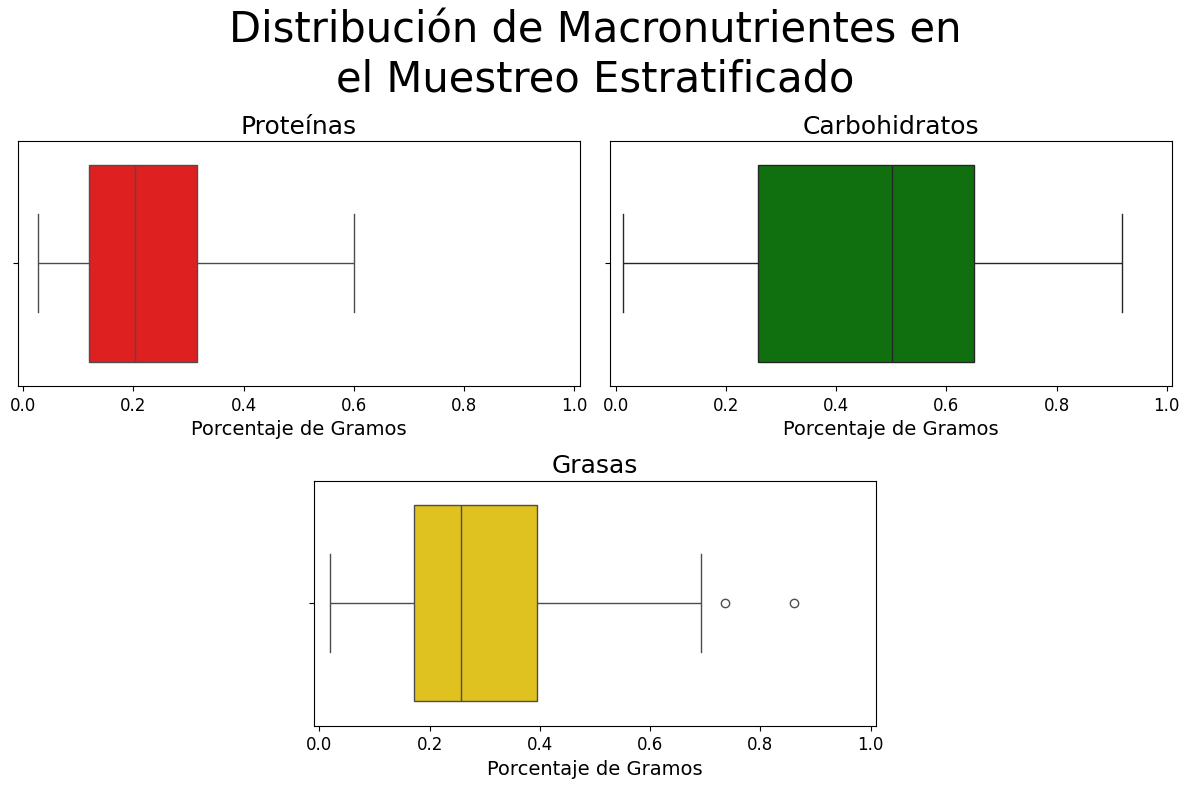
\includegraphics[width=0.75\textwidth]{Resources/3_02_plot_01.png}
        \end{center}

    \subsection{Intervalos de Confianza}
        En cada muestreo, se determinaron los intervalos 
        con los niveles de confianza del $85\%$, $95\%$ y $99\%$, 
        y en cada intervalo se determinó si la media poblacional de 
        la proporción de carbohidratos (siendo igual a $0.433471$) 
        pertenece al intervalo construido.

    \subsubsection{Muestreo Aleatorio}
        Los intervalos construidos son:
        \begin{center}
            \begin{tabular}{|c|c|c|}
                \hline
                Nivel de Confianza & Límite Inferior & Límite Superior \\
                \hline
                $85\%$ & 0.395173 & 0.495454 \\
                $95\%$ & 0.377046 & 0.513581 \\
                $99\%$ & 0.355595 & 0.535032 \\
                \hline
            \end{tabular}
        \end{center}
        Se puede observar que la media poblacional se 
        encuentra en todos los intervalos construidos 
        a partir del muestreo aleatorio.
            
    \subsubsection{Muestreo Estratificado}
        Los intervalos construidos son:
        \begin{center}
            \begin{tabular}{|c|c|c|}
                \hline
                Nivel de Confianza & Límite Inferior & Límite Superior \\
                \hline
                $85\%$ & 0.410682 & 0.505602 \\
                $95\%$ & 0.393524 & 0.522760 \\
                $99\%$ & 0.373220 & 0.543064 \\
                \hline
                \end{tabular}
        \end{center}
        Se pueden crear dos observaciones: La media 
        poblacional se encuentra en todos los intervalos 
        construidos; éstos son más pequeños en comparación 
        con los del muestreo aleatorio (esto debido a la 
        desviación estándar).

    \subsection{Hipótesis}
        Si se usara la media como indicativo para determinar 
        si un muestreo es representativo, entonces: ¿Los muestreos 
        realizados son representativos? De forma equivalente, ¿Las 
        medias muestralas de la proporción de carbohidratos difieren 
        significativamente de la media poblacional?
        
\newpage

\printbibliography[heading=bibintoc,title={Referencias Bibliográficas}]

\end{document}